\documentclass[10pt]{article}
\usepackage[utf8]{inputenc}

%Márgenes y tipo de hoja
\usepackage{geometry}
\geometry{letterpaper,portrait,
rmargin=20mm, 
lmargin=20mm,
bmargin=20mm,
tmargin=0mm,
headheight=0mm}
% \renewcommand{\headrulewidth}{1pt}
\usepackage{graphicx}
\usepackage{wrapfig}
\usepackage{float}

% Logos
\usepackage{fontawesome}

%Header
\usepackage{xcolor}
\usepackage{fancyhdr}
\pagestyle{fancy}
\fancyhf{}

% Tipo de letra y color
\usepackage{PTSansNarrow} 
\renewcommand*\familydefault{\sfdefault}
\usepackage[T1]{fontenc}
\usepackage{xcolor}
\usepackage{anyfontsize}

% Indentacion de parrafos completos
\usepackage{changepage}

% Paquete para columnas multiples
\usepackage{multicol}
\setlength{\columnsep}{40pt}
 \usepackage{vwcol} 

% Indentacion y otras longitudes
\setlength{\parindent}{0pt}
\setlength{\parskip}{10pt}
\renewcommand{\baselinestretch}{1}

% Figura
\usepackage{tikz}

% Hipervinculos
\usepackage{hyperref}

\begin{document}

\begin{tikzpicture}[remember picture,overlay]
   \node[anchor=north,inner sep=0pt] at (current page.north)
  \draw[blue, very thick] (-5,-3.1) rectangle (50,5);
  \filldraw[fill=blue!50!black, draw=blue!50!black](-5,-3.1) rectangle (50,5);
\end{tikzpicture}
\begin{tikzpicture}[remember picture,overlay]
    \node[anchor=north east,inner sep=0pt] at (current page.north east)
    {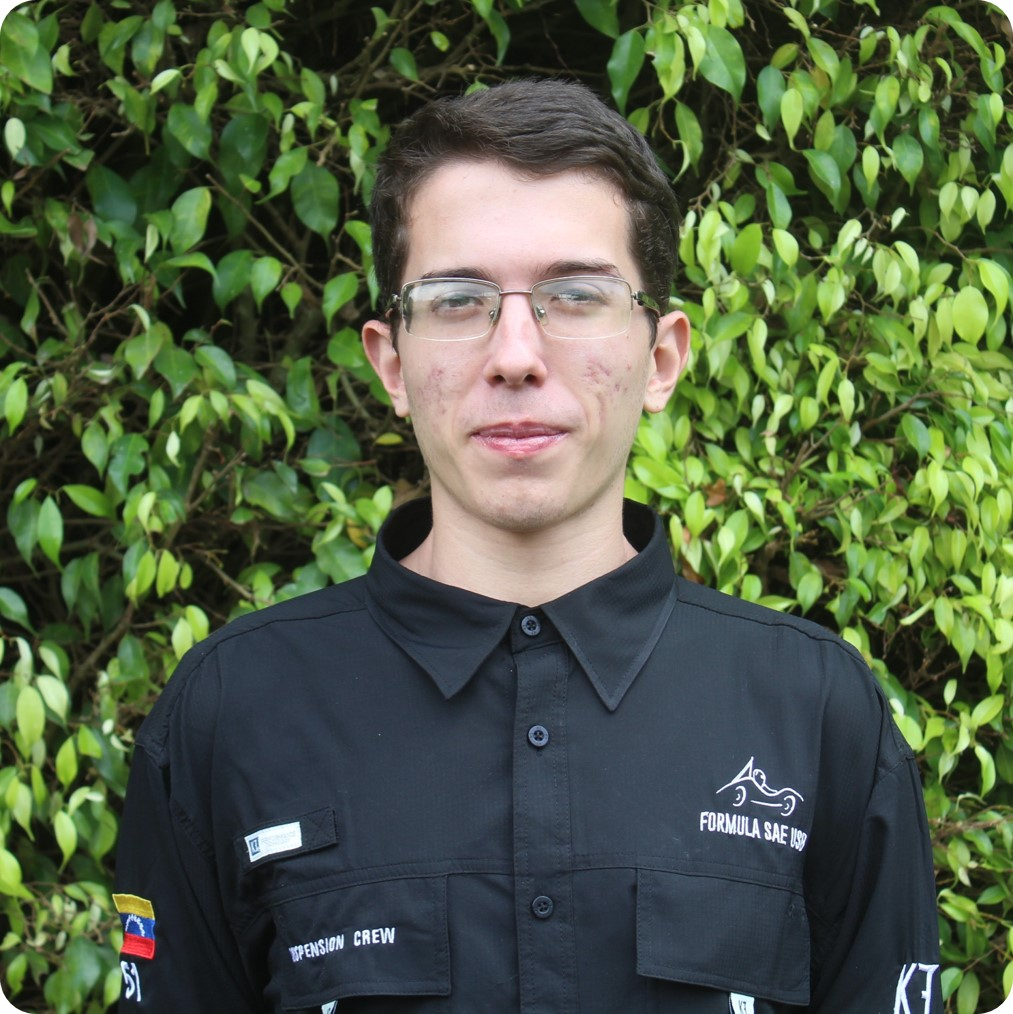
\includegraphics[scale=0.2]{foto/foto_perfil.JPG}};
\end{tikzpicture}

\begin{center}
    \color{white}
    {\fontsize{40}{60}\selectfont Jesús \textbf{Pereira}}\vspace{4pt}\\
    \faMapMarker\hspace{3pt}Caracas\hspace{5pt}/\hspace{5pt}Venezuela\hspace{25pt}| \hspace{25pt}\faMobile\hspace{2pt} +58 424 1234715\hspace{25pt}|
    \hspace{25pt}\faChain\hspace{2pt}\href{https://jesusepp.github.io/}{jesusepp.github.io}\\\vspace{2pt}
    \faEnvelope\hspace{2pt}jesusepereira@gmail.com\hspace{25pt}|
    \hspace{25pt}\faLinkedinSquare\hspace{3pt}\href{https://www.linkedin.com/in/jeppires/}{/in/jeppires/}\hspace{25pt}|
    \hspace{25pt} \faGithubSquare\hspace{3pt}\href{https://github.com/jesusepp}{/jesusepp}
\end{center}

\vspace{20pt}

\begin{multicols}{2}
    \begin{LARGE}
        \color{blue!50!black}Habilidades\par
    \end{LARGE}
    \begin{vwcol}[widths={0.4,0.6},
 sep=0cm,rule=0pt,indent=0em,lines=10]
        \textbf{Lenguajes de \\
        Programación}\par\hfill\\
        \textbf{Otros Lenguajes}\par\hfill\\
        \textbf{Programas y\\ plataformas}\par\hfill\\\hfill\\\hfill\\
        MATLAB, Python, JavaScript PHP, SQL, C++.\par\hfill\\
        Tex, HTML, CSS.\par\hfill\\
        SolidWorks, ANSYS Mechanical, ANSYS Fluent, MATLAB, OverLeaf, Excel, PowerPoint, Word, Google Docs.\par
    \end{vwcol}
    \columnbreak
    \begin{LARGE}
        \color{blue!50!black} Información Personal\par
    \end{LARGE}
    Actual estudiante de 10mo trimestre en Ingeniería Mecánica, miembro del equipo de fórmula SAE de la universidad Simón Bolívar, apasionado del aprendizaje y capaz de resolver problemas que requieran trabajo en equipo y cooperación.\par
    \begin{LARGE}
        \color{blue!50!black} Idiomas\par
    \end{LARGE}
    \begin{vwcol}[widths={0.235,0.765},
 sep=.8cm,rule=0pt,indent=0em,lines=4]
        \textbf{Español}\\
        \textbf{Inglés}\\
        \textbf{Alemán}\\
        \textbf{Portugués}\\
        Nativo\\
        Avanzado\\
        Básico\\
        Básico\\
    \end{vwcol}
\end{multicols}

\begin{LARGE}
        \color{blue!50!black} Cursos\par
\end{LARGE}
    
\begin{multicols}{2}
    \begin{vwcol}[widths={0.235,0.765},
 sep=.8cm,rule=0pt,indent=0em,lines=9]
        \hspace{5pt}Oct/2019\\
        \hfill\\
        \hfill\\
        \hspace{5pt}Abr/2020\\
        \hfill\\
        \hfill\\
        \hspace{5pt}May/2020\\
        \hfill\\
        \hfill\\
        CSWA, SolidWorks Associated. Credencial: \href{https://cv.virtualtester.com/qr/?b=SLDWRKS&i=C-4JDU269MA5}{\textbf{C-4JDU269MA5}}\par\hfill\\
        Certificación en el EF SET con 80/100. Credencial: \href{https://www.efset.org/cert/oZC3oZ}{\textbf{EF-SET}}\par\hfill\\
        Introduction to Programming with MATLAB. Credencial: \href{https://www.coursera.org/account/accomplishments/verify/E63RKFRUKWEU}{\textbf{E63RKFRUKWEU}}\par\hfill\\
    \end{vwcol}
    \columnbreak
    \begin{vwcol}[widths={0.235,0.765}, sep=.8cm,rule=0pt,indent=0em,lines=9]
        \hspace{5pt}Jul/2020\\
        \hfill\\
        \hfill\\
        \hspace{5pt}Jul/2020\\
        \hfill\\
        \hfill\\
        \hspace{5pt}Ago/2020\\
        \hfill\\
        \hfill\\
        Statistics with Python Specialization. Credencial: \href{https://www.coursera.org/account/accomplishments/specialization/certificate/NE5BJHUXH5VM}{\textbf{NE5BJHUXH5VM}}\par\hfill\\
        Engineering Project Management Specialization. Credencial: \href{https://www.coursera.org/account/accomplishments/specialization/certificate/YMNNPDXQL97L}{\textbf{YMNNPDXQL97L}}\par\hfill\\
        SQL for Data Science. Credencial: \href{https://www.coursera.org/account/accomplishments/certificate/MSH6GML4W8AM}{\textbf{MSH6GML4W8AM}}\par\vspace{5px}
    \end{vwcol}
\end{multicols}

\begin{LARGE}
    \color{blue!50!black} Educación\par
\end{LARGE}
\begin{multicols}{2}
     \begin{vwcol}[widths={0.4,0.6}, sep=.2cm,rule=0pt,indent=0em,lines=4]
    \hspace{5pt}Abr/2016 - Presente\\
    \hfill\\
    \hfill\\
    \hfill\par
    \textbf{Ingeniería Mecánica}\\
    Universidad Simón Bolívar\\
    160 unidades-crédito (73\% del total)\\
    Índice Académico: 4.92/5.00
    \end{vwcol}
\end{multicols}


\begin{LARGE}
    \color{blue!50!black} Experiencia Laboral\par
\end{LARGE}

\begin{vwcol}[widths={0.235,0.765},
 sep=.8cm,rule=0pt,indent=0em,lines=7]
    \hspace{5pt}Jul/2020 - Presente\par
    \hfill\\
    \hfill\\
    \hfill\\
    \hfill\\
    \hfill\\
    \hfill\\
    \textbf{Director Técnico / Director de las divisiones de Chasis y Frenos}
    \hfill
    \href{http://fsaeusb.com.ve/}{\color{blue!50!black}\textbf{FSAE USB}}\\
    \vspace{5pt}
    El director técnico es el encargado de dirigir y controlar las acciones asociadas a las divisiones técnicas del equipo. Esta posición requiere buen liderazgo, planificación y buena comunicación con cada uno de los encargados de división. Motorsports, dinámica vehicular, diseño asistido por computador (CAD), e ingeniería asistida por computador (CAE) son algunos de las áreas técnicas que esta posición requiere. Adicionalmente, este año los cargos de director de chasis y frenos fueron tomados por el director técnico.\par
\end{vwcol}
\clearpage
\hfill\\
\hfill\\

\begin{vwcol}[widths={0.235,0.765},
 sep=.8cm, rule=0pt,indent=0em,lines=8]
    \hspace{5pt}Jul/2019 - Jul/2020\par
    \hfill\\
    \hfill\\
    \hfill\\
    \hfill\\
    \hfill\\
    \hfill\\
    \hfill\\
    \textbf{Director de la división de Chasis}
    \hfill
    \href{http://fsaeusb.com.ve/}{\color{blue!50!black}\textbf{FSAE USB}}\\
    \vspace{5pt}
    Como director de Chasis, se heredan las responsabilidades de diseñar, construir y verificar los diversos sistemas encargados para esta división, entre ellos el frame y sus conexiones con los diversos sistemas del carro y los elementos de seguridad requeridos por la competencia (atenuador de impacto, material absorbente de impactos, entre otros). Es de suma importancia para este cargo tener una buena comunicación con los demás jefes de división, ya que Chasis se encarga de unirlos y evitar que puedan existir problemas entre ellas.\par
\end{vwcol}

\begin{vwcol}[widths={0.235,0.765},
 sep=.8cm, rule=0pt,indent=0em,lines=6]
    \hspace{5pt}Jul/2018 - Jun/2019\par
    \hfill\\
    \hfill\\
    \hfill\\
    \hfill\\
    \hfill\\
    \textbf{Miembro de la división de Suspensión}
    \hfill
    \href{http://fsaeusb.com.ve/}{\color{blue!50!black}\textbf{FSAE USB}}\\
    \vspace{5pt}
    Esta división es la encargada del diseño, construcción y seteo del sistema de suspensión de un prototipo Formula Student construido por FSAE USB. Junto con los demás miembros de la división, se trabajó en equipo para lograr un sistema funcional, con ayuda de softwares de diseño como SolidWorks, y herramientas de taller como tornos, fresadoras, y equipos de mecánica básicos (llaves, tornillería, entre otros).\par
\end{vwcol}

\begin{LARGE}
    \color{blue!50!black} Proyectos\par
\end{LARGE}

\begin{vwcol}[widths={0.235,0.765},
 sep=.8cm, rule=0pt,indent=0em,lines=6] 
\hspace{5pt}Jun/2020 - Jul/2020\par
    \hfill\\
    \hfill\\
    \hfill\\
    \hfill\\
    \hfill\\
    \textbf{Página Web}\hfill \href{https://jesusepp.github.io/}{\color{blue!50!black}\textbf{jesusepp.github.io}}\\
    \vspace{5pt}
    Durante la cuarentena del 2020, comencé a aprender sobre desarrollo web, principalmente por curiosidad. Pero, como un objetivo personal, para practicar mis nuevas habilidades, comencé este proyecto, junto con mi amigo José, para desarrollar un sitio web personal que sirva de fuente de información detallada e ilustrativa sobre mi.\par
\end{vwcol}

\begin{vwcol}[widths={0.235,0.765},
 sep=.8cm, rule=0pt,indent=0em,lines=5] 
\hspace{5pt}Abr/2020\par
    \hfill\\
    \hfill\\
    \hfill\\
    \hfill\\
    \textbf{Buscaminas en Python}\hfill \href{https://github.com/jesusepp/minesweeper}{\color{blue!50!black}\textbf{/jesusepp/minesweeper}}\\
    \vspace{5pt}
    
    A través del lenguaje de programación Python, y con la finalidad de probar las capacidad adquiridas para desempeñarse con este lenguaje, se realizó una versión para el terminal de este popular juego. Los resultados fueron aceptables.\par
\end{vwcol}

\begin{vwcol}[widths={0.235,0.765},
 sep=.8cm, rule=0pt,indent=0em,lines=8] 
\hspace{5pt}Ene/2020 - Abr/2020\par
    \hfill\\
    \hfill\\
    \hfill\\
    \hfill\\
    \hfill\\
    \hfill\\
    \hfill\\
    \textbf{Virtual Formula 2020}\hfill \href{https://www.vi-grade.com/en/about/virtual_formulas/virtual-formula-2020/?#virtualformula2020}{\color{blue!50!black}\textbf{vi-grade.com - 2020 Results}}\\
    \vspace{5pt}
    Esta es una competencia virtual, asociada a Formula SAE, y este año nuestro equipo decidió participar en él (conmigo a cargo). Esta competencia se basa en la simulación de un vehículo monoplaza, por medio del Virtual Race Car software (simulador de vuelta) de VI-grade, donde cada equipo tenía que setear el vehículo para hallar la configuración que obtuviese los mejores tiempos, dentro de los parámetros de la competencia. Terminamos de 20/35, siendo esta nuestra primera vez participando y utilizando este software.\par
\end{vwcol}
\end{document}
